\documentclass[
  10pt,               % 120% Schriftgrösse
  oneside,            % einsitiger Druck
  a4paper,            % A4
  titlepage,          % inklusive Titelpage
  pointlessnumbers,	  % Kein Punkt hinter der Kapitelnummerierung
  halfparskip,        % Europäischer Satz mit abstand zwischen Absätzen
  pdftex,             % Direkt ins Pdf übersetzen, keine Kapitel
  liststotoc,         % Inhaltsverzeichnis inkl. Abbildungsverzeichnis
  bibtotoc]{scrreprt} % Inhaltsverzeichnis inkl. Literaturverzeichnis

%%%%%%%%%%%%%%%%%%%%%%%%%
% Allgemeine Packete    %
%%%%%%%%%%%%%%%%%%%%%%%%%

% Neue Rechtschreibung
\usepackage[german, ngerman]{babel}

% UTF 8
\usepackage[utf8]{inputenc}
\usepackage{nicefrac}
\usepackage{multirow}

% Ausgabefonts
\usepackage[T1]{fontenc}

% Euro Symbol (\texteuro}
\usepackage{textcomp}

% für die Gesamtseitenzahl
\usepackage{totpages}

% Paket für Farben
\usepackage{color}

% Bilder
%\usepackage{graphicx}

% Fliesstext um Bilder
\usepackage{wrapfig}

% Tabellen mit definierter Breite und zentriert
\usepackage{array}

\newcolumntype{x}[1]{%
>{\centering\hspace{0pt}}p{#1}}%

% Glossar alt
%\usepackage[style=super, header=none, border=none, number=none, cols=2, toc=true]{glossary}
%\makeglossary

% Glossar neu
\usepackage[xindy]{glossaries}
%\usepackage{glossaries}
%\makeglossaries
%\printglossaries

% mehrere Befehle für die Tabellen
\usepackage{booktabs}

%Packet für absolut Positionierte Textboxen
\usepackage[absolute]{textpos} %showboxes zum besseren positionieren

% Packet für Boxen
%\usepackage{framed}

% Initialen
%\usepackage{lettrine}
%\DeclareFixedFont{\Yinit}{U}{yinit}{m}{n}{16}


%%%%%%%%%%%%%%%%%%%%%%%%%
% Seiteneinstellungen   %
%%%%%%%%%%%%%%%%%%%%%%%%%
\usepackage[
  portrait,
%   twoside,
  left=40mm,
  top=20mm,
  textwidth=145mm,
  textheight=252mm,
  %head=15mm,
  head=15mm,
  headsep=5mm,
  foot=8mm
]{geometry}

% Text muss nicht umbedingt bis zur Fusszeile reichen
\raggedbottom

%\usepackage[cam,axes,a3,center]{crop}
%\usepackage[frame,a4,center]{crop}

%%%%%%%%%%%%%%%%%%%%%%%%%
% Schriftart            %
%%%%%%%%%%%%%%%%%%%%%%%%%

%\usepackage{courier}  % Courier für Code verwenden
%\usepackage{helvet}   % Helvetica
% Helvetic als Font verwenden
%\renewcommand{\familydefault}{\sfdefault}


%%%%%%%%%%%%%%%%%%%%%%%%%
% Mathematik Packete    %
%%%%%%%%%%%%%%%%%%%%%%%%%

% Verbesserte Mathematik Satz
\usepackage{amsmath}

% Zahlenmenngen in der Mathematik
\usepackage{amssymb}

% Times New Roman für Mathematik
\usepackage{mathptmx}


%%%%%%%%%%%%%%%%%%%%%%%%%
% Inhaltsverzeichnis    %
%%%%%%%%%%%%%%%%%%%%%%%%%
% Punkte im Inhaltsverzeichnis bei Sections
\usepackage{tocloft}
\renewcommand{\cftsecdotsep}{4.5}

%%%%%%%%%%%%%%%%%%%%%%%%%
% Literaturverzeichnis  %
%%%%%%%%%%%%%%%%%%%%%%%%%

%\usepackage[ngerman,ref]{backref}
%\renewcommand{\backrefpagesname}{Zitiert auf S.}
%renewcommand{\refname}{Quellenverzeichnis}

%%%%%%%%%%%%%%%%%%%%%%%%%
% Anhang			    %
%%%%%%%%%%%%%%%%%%%%%%%%%

\newcommand{\anhang}[1]{
	%\setsection{1}
    \setcounter{page}{1}
	\input{#1}
	\newpage
}

%%%%%%%%%%%%%%%%%%%%%%%%%
% Source Code Packete   %
%%%%%%%%%%%%%%%%%%%%%%%%%

% Codesegmente
\usepackage{listings}
\definecolor{darkblue}{rgb}{0,0,0.6}
\definecolor{darkred}{rgb}{0.6,0,0}
\definecolor{darkgreen}{rgb}{0,0.6,0}
\definecolor{red}{rgb}{0.98,0,0}
\lstloadlanguages{C,C++} % entsprechende Sprachen werden hier schon mal geladen, damit das Übersetzen schneller geht
\lstset{%
  language=C,
  basicstyle=\footnotesize\ttfamily,
  commentstyle=\itshape\color{darkgreen},
  keywordstyle=\bfseries\color{darkblue},
  stringstyle=\color{darkred},
  showspaces=false,
  columns=fixed,
  numbers=left,
  frame=none,
  numberstyle=\tiny,
  breaklines=true,
  showstringspaces=false,
  xleftmargin=1cm,
  tabsize=2
}%


%%%%%%%%%%%%%%%%%%%%%%%%%
% Makros                %
%%%%%%%%%%%%%%%%%%%%%%%%%

% Makros
\newcommand{\redbox}[1]
{\vspace*{2mm} \\ \fboxsep5mm \fboxrule0.5mm \fcolorbox{red}{white}{\parbox{1.5cm}{
\includegraphics[width=1cm]{Achtung.pdf}}\parbox{13cm}{\textcolor{black}{#1}
}}\vspace*{2mm}\\}

\newcommand{\redboxtitle}[2]
{\vspace*{2mm} \\ \textcolor{red}{\bfseries #1\smallskip} \\ \fboxsep5mm \fboxrule0.5mm \fcolorbox{red}{white}{\parbox{1.5cm}{
\includegraphics[width=1cm]{Achtung.pdf}}\parbox{13cm}{\textcolor{black}{#2}
}}\vspace*{2mm}\\}

% Fuer die Minipage um eine Tabelle und Abbildung nebeneinander Setzen
\makeatletter
\newcommand{\setcaptype}[1]{\renewcommand{\@captype}{#1}}
\makeatother


%%%%%%%%%%%%%%%%%%%%%%%%%
% Kopf und Fusszeile    %
%%%%%%%%%%%%%%%%%%%%%%%%%
% 7. Kopf und Fusszeilen
\usepackage{totpages}               % Paket für die Gesamtseitenzahl
\usepackage{scrpage2}
\pagestyle{scrheadings}
\renewcommand*{\chapterpagestyle}{scrheadings}
\clearscrheadfoot
%\setkomafont{pagefoot}{\normalfont\sffamily}
\automark[]{chapter}
%\ihead{NTB-Robotersteuerung}
\ihead{VT1: EEROS Sequencer}
\ohead{\headmark}
\setheadsepline{0.5pt}[\color{HeadBlue}] 
%\ifoot{Benno Jung • Michael Krähenbühl • Martin Züger}
\cfoot{- \thepage{} -}
%\setfootsepline{0.5pt}
%%Kopf- und Fusszeile
\definecolor{HeadBlue}{rgb}{0,0.41,0.71}
\definecolor{FootBlack}{rgb}{0,0,0}
\addtokomafont{pagehead}{\color{HeadBlue}} 
\addtokomafont{pagefoot}{\color{FootBlack}}
%\usepackage{eso-pic}
%\usepackage{scrpage2}
%\usepackage{extramarks}
\usepackage[final]{pdfpages}
%%\pagestyle{scrheadings}
%%\clearscrheadfoot
%% Schriftart auf die Normale Schrift setzen
%%\setkomafont{pagefoot}{\normalfont\sffamily}
%%\automark[]{section} % \leftmark zeigt die aktuelle Section an, \rightmark bleibt leer
%
%%Kopfzeile
%%\ihead{NTB}
%%\ohead{\leftmark}
%%\lehead{\hspace*{1cm}\begin{large}\leftmark\end{large} \AddToShipoutPicture*{%
%%  \AtPageUpperLeft{\put(0,\LenToUnit{-9.4mm}){%
%%    \colorbox{HeadBlue}{\parbox[t][6mm]{1.8cm}{\ }}%
%%    \colorbox{black}{\parbox[t][6mm]{0.1cm}{\ }}}}}}
%%\rohead{\begin{large}\leftmark\end{large}\hspace*{1cm} \AddToShipoutPicture*{%
%%  \AtPageUpperLeft{\put(\LenToUnit{\paperwidth},\LenToUnit{-9.4mm}){\kern-2.3cm%
%%    \colorbox{black}{\parbox[t][6mm]{0.1cm}{\ }}%
%%    \colorbox{HeadBlue}{\parbox[t][6mm]{1.8cm}{\ }}}}}}
%%\rehead{\begin{large}NTB\end{large}}
%%\lohead{\begin{large}NTB\end{large}}
%%\setheadsepline{1.2pt}
%\usepackage{ifthen}
%\newboolean{SectionOnPage}
%\renewcommand{\sectionmark}[1]{\setboolean{SectionOnPage}{true}\markboth{#1}{#1}}
%\newcommand{\headerblackbox}{\colorbox{black}{\parbox[c][6mm]{0.1cm}{\ }}}
%\newcommand{\headerbluebox}[1]{\colorbox{HeadBlue}{\parbox[c][6mm]{1.8cm}{%
%%       \ifnum\value{section}>0
%%         \ifthenelse{true}{H}{#1\textbf{\begin{large}\color{white}{\sffamily{\arabic{section}}}\end{large}}}
%%       \else
%          #1 \textbf{\begin{large}\color{white}{\sffamily{\ }}\end{large}}
%%       \fi
%}}}
%\newcommand{\headerbluetext}[1]{\textbf{\begin{large}\color{HeadBlue}{#1}\end{large}}}
%%\newcommand{\headerNTB}{\headerbluetext{NTB}}
%\newcommand{\headerNTB}{\includegraphics[height=1.2cm]{ntb}}
%\newcommand{\headerleftmark}{\headerbluetext{\firstleftmark}}
%
%\lehead{\hspace*{5mm}\headerleftmark \AddToShipoutPicture*{%
%  \AtPageUpperLeft{\put(0,\LenToUnit{-13.4mm})}}}
%
%\rohead{\headerleftmark \hspace*{5mm} \AddToShipoutPicture*{%
%  \AtPageUpperLeft{\put(\LenToUnit{\paperwidth},\LenToUnit{-13.4mm})}}}
%
%
%%\rehead{\headerNTB}
%%\lohead{\headerNTB}
%\rehead{Seite \thepage{}}
%\setheadsepline{0.8pt}
%\renewcommand*{\chapterpagestyle}{scrheadings}
%%\setheadsepline{0.5pt}[\color{blue}]
%
%%Fusszeile
%%\ifoot{Marcel Gehrig, Egemen Yesil}
%%\cfoot{\today}
%\cfoot{- \thepage{} -}
%%\ofoot{\thepage{} / \ref{TotPages}}
%%\setfootsepline{0.5pt}

%%%%%%%%%%%%%%%%%%%%%%%%%
% Informationen         %
% über den Autor        %
%%%%%%%%%%%%%%%%%%%%%%%%%

\title{VT1: EEROS Sequencer 2017}
\author{Marcel Gehrig}
\date{Januar 2017}


%%%%%%%%%%%%%%%%%%%%%%%%%
% Pdf Einstellungen     %
%%%%%%%%%%%%%%%%%%%%%%%%%

% Paket für Links innerhalb des PDF Dokuments und Pdf Informationen
\definecolor{LinkColor}{rgb}{0,0,0}
\usepackage[
  pdftitle={VT1 EEROS Sequencer},
  pdfauthor={Marcel Gehrig},
  pdfcreator={Texmaker},
%  pdfsubject={VT1 EEROS Sequencer},
  pdfsubject=pdftitle,
  pdfkeywords={Schlussbericht,Vertiefungsarbeit,EEROS,Sequencer,C++,Roboter Steuerung}]{hyperref}
\hypersetup{colorlinks=true,
  linkcolor=LinkColor,
  citecolor=LinkColor,
  filecolor=LinkColor,
  menucolor=LinkColor,
  urlcolor=LinkColor}

% Packet um Dateien in das PDF einzubetten
\usepackage{attachfile}
\usepackage{pdfpages}
%%%%%%%%%%%%%%%%%%%%%%%%%
% Farben                %
%%%%%%%%%%%%%%%%%%%%%%%%%

\definecolor{Blue}{rgb}{0,0,1}
\definecolor{Red}{rgb}{1,0,0}
\definecolor{Green}{rgb}{0,1,0}

%%%%%%%%%%%%%%%%%%%%%%%%%%%
%%%%%%%%%%%%%%%%%%%%%%%%%%%
%% ACHTUNG:              %%
%% Informationen über    %%
%% den Autor müssen in   %%
%% folgenden Abschnitten %%
%% angepasst werden:     %%
%%                       %%
%% - PDF EINSTELLUNGEN   %%
%% - KOPF UND FUSSZEILE  %%
%% - AUTOR               %%
%%%%%%%%%%%%%%%%%%%%%%%%%%%

%Tiefe der nummerierten Ebene
\setcounter{tocdepth}{4} %Anzeigetiefe im Inhaltsverzeichniss
\setcounter{secnumdepth}{4} %Nummerierungstiefe
\renewcommand*{\chapterpagestyle}{scrheadings} %Kopfzeile auch bei \chapter
\renewcommand*{\chapterheadstartvskip}{\vspace*{-\topskip}}  %Abstand korrigieren von Kopfzeile zu \chapter
\setlength{\cftbeforetoctitleskip}{-2mm} 
\setlength{\cftaftertoctitleskip}{0.5mm}
\usepackage{placeins} %um floatbarrier zu benutzen
%\usepackage{mathtext}

%Pfad für die Bilder Festlegen
%\graphicspath{{Bilder/},{Icons/},{Logo/},{Template/},{Ismages/},{}}
\graphicspath{{images_P/},{}}
\newglossaryentry{MMU}
{
  name=MMU,
  description={ist die Memory Management Unit. Sie übersetzt die virtuellen Addressen der CPU in die Physikalischen Addressen. Eine MMU wird für einen externen Memory Mapped Bus notwendig.}
}
%%Grosser Zeilenabstand für Korrektur
% \usepackage{setspace}
% \linespread{2}

%%%%%%%%%%%%%%%%%%%%%%%%%
% Dokument              %
%%%%%%%%%%%%%%%%%%%%%%%%%
\begin{document}
	\renewcommand{\thepage}{\roman{page}}
	\renewcommand{\bibname}{Quellenverzeichnis}
%	
\begin{titlepage}
	\setlength{\TPHorizModule}{\paperwidth}
	\setlength{\TPVertModule}{\paperheight}
	\begin{textblock}{0.95}[0.5,0](0.5,0.04)
	\makebox{\includegraphics[width=\textwidth]{images/iduna_logo}}
	\end{textblock}
	\begin{textblock}{0.3}[0,0](0.68,0.03)
	\makebox{\includegraphics[width=5.5cm]{images/ntb.png}}
	\end{textblock}
    \vspace*{6cm}
    \begin{center}
    	\Huge{\color{HeadBlue}{Basisstation zu elektrophysiologischem Mini-Datenlogger\\}}
		\vspace*{2cm}
		\normalsize
      	{\color{HeadBlue}{\sffamily{
      		\textbf{Bachelorarbeit 2010} \\
      		\textbf{im Bereich Medizintechnik} \\
      		\vspace*{1cm}
      		von \\
			~\newline
      		\textbf{Alexander Bucher}\\
      		\textbf{Philippe Rüesch}
      		}}}\\
		\vspace*{2cm}      	
		\includegraphics[height=4cm]{images/logo_valens}


    \vspace*{1.5cm}
    \color{HeadBlue}
    \begin{tabular}{p{4cm}l}
      Referent: & Dr. Urs Moser \\
      Korreferent: & Dr. Andreas Zogg \\
      Abgabedatum: & 13. August 2010
    \end{tabular}\\
    \end{center}
  \end{titlepage}




%	\newpage
%	
\chapter*{Zusammenfassung}
Im Auftrag des Industriepartner Variosystems wurde ein kostengünstiger, auf dem BeagleBone Black basierter Platinencomputer entwickelt. Der BeagleBone Black, im weiteren Text als BBB bezeichnet, ist ein vollständiger Computer für Linux-basierte Betriebssysteme. Standardmässig wird es mit dem Betriebssystem Debian ausgeliefert, welches für diese BA ebenfalls benutzt wird. Im Verlauf dieser Arbeit wurden insgesamt 5 Exemplare hergestellt, die alle bei Variosystems bestückt wurden. Mit einem Cape, einer aufsteckbaren Platine für den BBB, wurde der Computer mit WLAN, Bluetooth Low-Energy, GSM/GPRS und einem Touchscreen ergänzt. Dieses Cape ist nicht nur mit dem von uns gebauten BBB-Derivat kompatibel, sondern auch mit dem kommerziell erhältlichen, originalen BBB. Die Kombination des BBB mit dem Cape wird im Folgenden Communication-Bone, oder kurz ComBone genant. Der Name ist eine Wortkombination des englischen Wortes "Communication" \ für die Kommunikationsfähigkeit des Capes über verschiedene Kanäle, sowie dem Wort "Bone", welches bereits im Namen des originalen BBB genutzt wird.

Bei der Entwicklung der Hard- und Software ist darauf geachtet worden, dass die einzelnen Funktionen möglichst modular sind. Wenn bestimmte Funktionen nicht benötigt werden, wie zum Beispiel der HDMI Anschluss des BBB oder die WLAN-Funktion des Capes, können die entsprechenden Bauteile bei der Produktion einfach nicht bestückt werden. Dies kann, besonders bei grösseren Stückzahlen, viel Geld sparen. Des Weiteren können auch einige Module, beziehungsweise Funktionen, einfach kopiert und in anderen Projekten verwendet werden.

Ein möglicher Einsatzbereich dieses Computers mit dem Cape ist die Verbindung von einem Gerät, wie etwa ein Sensor oder ein abgelegener Stromgenerator, mit dem Internet. Der ComBone kann sich mit einer LAN-Verbindung, mit WLAN oder über das mobile GSM Netz, wie es auch ein Mobiltelefon verwendet, ins Internet einwählen. Dies macht den ComBone zu einem  hochflexibles Gerät, welches diverse Einsatzmöglichkeiten hat.





\section*{Abstract}
%TODO Englischübersetzung

	\newpage
	\makeatletter
	\addtocontents{toc}{\protect\thispagestyle{scrheadings}}
	\renewcommand{\tableofcontents}{\section*{\contentsname} \pagestyle{scrheadings} \@starttoc{toc}}
	\makeatother
	\tableofcontents
	\newpage
	\renewcommand{\thepage}{\arabic{page}}
	\setcounter{page}{1}
	
	\chapter{Einleitung}


\section{Industriepartner}
Variosystems ist ein international tätiges Elektronikdienstleistungsunternehmen mit 1100 Mitarbeitern. Es stellt elektronische Baugruppen und Geräte her. In den Produktionsstätten werden PCB mit Bauteilen bestückt und verlötet. 
%\cite{variosystems} 

In dieser Arbeit ist Variosystems nicht nur der Auftraggeber, sondern arbeitet auch aktiv mit. In vielen technischen Fragen haben die Ingenieure von Variosystems ihr Know-how eingebracht. Die PCBs für den BeagleBone Black wurden ebenfalls in einer Produktionsstätte von Variosystems bestückt.



\section{Motivation}
Variosystems bestückt nicht nur fremde PCBs, sie stellen auch eigene Produkte her. Einige dieser Produkte müssen, z. B. für Wartung und Systemüberwachung, mit dem Internet verbunden werden.

Eine mögliche Lösung wäre der BeagleBone Black (kurz BBB). Dieser kostengünstige Platinencomputer bringt neben USB und I$^2$C noch diverse andere Schnittstellen, die in der Elektronik üblich sind, mit. Allerdings hat der BBB weder WLAN noch Bluetooth Low Energy (kurz BLE) integriert. Ein weiteres Problem ist, dass das Produkt in grösseren Stückzahlen Lieferprobleme haben kann. Dies ist in der Vergangenheit bereits vorgekommen.

Wenn die Variosystems diesen Platinencomputer selbst herstellen könnte, wäre sie nicht mehr auf die Lieferbarkeit des BBB angewiesen. Zusätzlich würde die Möglichkeit bestehen, den Computer nach eigenen Wünschen zu modifizieren. So können zusätzliche Funktionen wie BLE und WLAN hinzugefügt, und nicht benötigte Funktionen weggelassen werden. Dies spart besonders dann Geld, wenn das Produkt in grossen Stückzahlen hergestellt wird.


\section{BeagleBone Black}
Der BeagleBone Black ist, obwohl er nur halb so gross ist wie eine Hand, ein vollständiger Computer. Er wird standardmässig mit einem Ubuntu Linux ausgeliefert. Direkt aus der Packung kann der BBB über ein HDMI Kabel an einen Bildschirm oder Fernseher angeschlossen und gestartet werden. Ein Cape, eine speziell für den BBB entwickelte Platine, kann den Platinencomputer um diverse Funktionen erweitern. In der Abbildung \ref{fig:BeagleBoneBlack} ist eine Fotografie des BBB zu sehen.

Neben einem Micro-HDMI-Anschluss hat der BBB auch noch einen LAN-Port, einen USB-Host und einen Mini-USB Client-Anschluss. Über den Mini-USB Client-Anschluss kann der BBB an einen anderen PC angeschlossen, und so programmiert werden. Der Host-Anschluss ist ein normaler USB-Port, der z. B. für eine Maus oder USB Stick verwendet werden kann.

Die Entwicklung des BBB wurde auf Massenproduktion und günstige Bauteile optimiert. Dies, und die grossen Stückzahlen, die produziert werden, führen zu einem sehr günstigen Produkt.

\begin{figure}[!ht]
\centering
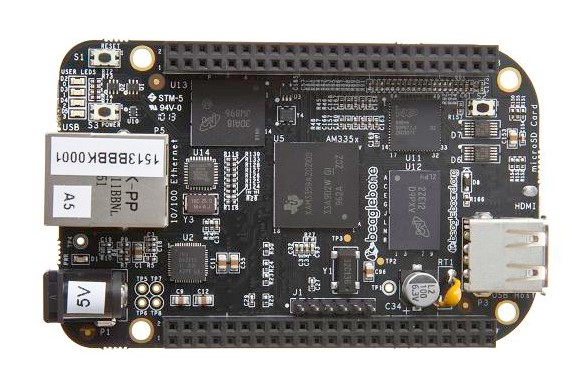
\includegraphics[angle=0,height=5cm]{images/BeagleBoneBlack.jpg}
\caption{Originaler BeagleBone Black}
\label{fig:BeagleBoneBlack}
\end{figure}


\section{Aufgabenstellung}
%Auftrag generell
Im Auftrag des Industriepartners Variosystems soll ein eigener, kostengünstiger und auf dem BeagleBone Black basierter Platinencomputer entwickelt werden. Dafür gilt es, ergänzend zu den eigentlichen Funktionen des BeagleBone Black, weitere Funktionen wie WLAN, Bluetooth Low-Energy, und GSM/GPRS zu integrieren. Zusätzlich soll ein TFT-Display mit einem kapazitivem Multi-Touch-Screen angeschlossen werden, welches von Variosystems zur Verfügung gestellt wird. Das Ganze soll dann als Einheit aufgebaut werden.

%Herstellbarkeit praktisch
Ziel der Arbeit ist es, dass Variosystems diesen Computer selber herstellen und nach Wunsch modifizieren kann. Die Produktionspläne sollen so aufbereitet werden, dass die benötigten PCBs bei einem PCB-Hersteller bestellt werden können. Die Bestückung der PCBs erfolgt dann bei Variosystems. Bei den Bauteilen ist ein besonderes Augenmerk auf die Lieferbarkeit zu werfen. Damit die Bauteile bestellt werden können, muss eine Bauteilliste, auch 'Bill of material' oder kurz BOM, erstellt werden. Diese Liste ist mit der Bestellnummer von üblichen Distributoren wie zum Beispiel Digi-Key oder Mouser zu ergänzen. Standartbauteile, wie etwa Widerstände, hat Variosystems auf Lager. Bei solchen Bauteilen muss auch die Artikelnummer von Variosystems für das entsprechende Bauteil in der BOM aufgeführt werden.

%Modularität, kritischer bereich, 
Die Hardware wie auch die Software sollen möglichst modular aufgebaut sein. Dies bedeutet für die Entwicklung der Hardware, dass alle Bauteile für eine bestimmte Funktion gruppiert und eindeutig erkennbar sein müssen. Ebenso sollen die Bauteile identifiziert werden, welche für die Lauffähigkeit des Computers unbedingt benötigt werden. Ein besonderes Augenmerk ist auf die Stellen zu werfen, bei denen die Leiterbahngeometrie relevant ist. Wie etwa bei der Hochgeschwindigkeitsschnittstelle zwischen Prozessor und RAM. Die Softwaretreiber sollen so geschrieben sein, dass die einzelnen Treiber ohne die anderen lauffähig sind. 

%Software
Zusätzlich zu den Treibern sollten auch Applikationen für die einzelnen Module entwickelt werden. Diese Applikationen sollen als Demonstration der Funktionen und als Vorlage für mögliche Anwendungen verwendet werden können.

	\chapter{Einleitung}

\section{Unterschiede zwischen ARM Cortex -A -R und -M}
\subsubsection{Cortex-A}
Sehr gut geeignet für die Verwendung mit einem vollen Betriebssystem wie Windows, Linux oder Android.
Die leistungstärksten ARM Cortex Prozessoren.


\subsubsection{Cortex-R}
Cortex-R werden entwickelt für Echtzeitanwendungen und Sicherheitskritische Applikationen wie Festplattenkontroller und medizinische Geräte.
Sie sind normalerweise nicht mit einer MMU ausgerüstet.
% und können deshalb nich mit einem Linux oder Windows verwendet werden.
Mit einer Taktrate von über 1GHz und einem sehr schnellen Interruptverhalten eignen sich Prozessoren mit einem Cortex-R sehr gut um auf externe Stimuli schnell zu reagieren.

\subsubsection{Cortex-M}
Cortex-M sind mit einer Taktrate um 200Mhz relativ langsam.
Sehr stromsparend und durch die kurze Pipeline haben sie eine deterministische und kurze Interrupt Verzögerung.
Die Prozessoren aus der Cortex-M Reihe unterstützen nur die Thumb Instruktionen und nicht die standard Arm Instruktionen.


\subsubsection{ARM Prozessoren ausserhalb der Cortex Reihe}
%TODO jahreszahl 2004?
Seit XXXX werden alle Kerne in eine der Cortex Gruppen eingeteilt.
Ältere Kerne haben namen wie z.b. ARM7 oder ARM1156T2F-S.
Da solche Designs aus einer Zeit vor XXXX stammen, gilt das Design als veraltet und wird bei dieser Arbeit nicht berücksichtigt.	%TODO jahreszahl


\subsubsection{Übersicht über die}

\begin{table}[]
\centering
\caption{My caption}
\label{my-label}
\begin{tabular}{|l|l|l|}
\hline
  & \textbf{Vorteile}                                                                                                                                                                                                                                    & \textbf{Nachteile}                                                                                                                                                                             \\ \hline
A & \begin{tabular}[c]{@{}l@{}}* Sehr Leistungsstartk\\ * Support für vollwertige Betriebssysteme\\ * Grosse Variation erhältich (Energiesparend /\\  sehr Leistungsstark)\\ * Reichhaltiger Funktionsumfang\\ * NEON und FPU Unterstützung\end{tabular} & \begin{tabular}[c]{@{}l@{}}* Langsamer Context-Switch\\ * Relativ hoher Stromverbrauch\\ * Relativ teuer\\ * Mit GPU erhältlich\\ * Keine DSP Unterstützung\\ * Keine HW-Division\end{tabular} \\ \hline
R & \begin{tabular}[c]{@{}l@{}}* Sehr gut geignet für Echtzeitanwendungen\\ * Sehr schneller Context-Switch\\ * DSP Unterstützung\end{tabular}                                                                                                           & \begin{tabular}[c]{@{}l@{}}* Kleiner Funktionsumfang\\ * Nicht so leistungstark wie Cortex A\\ * Keine Linux Unterstützung\end{tabular}                                                        \\ \hline
M & \begin{tabular}[c]{@{}l@{}}* Sehr schneller Context-Switch\\ * Sehr energiesparend\\ * DSP Unterstützung\end{tabular}                                                                                                                                & \begin{tabular}[c]{@{}l@{}}* Geringe Rechenleistung\\ * Keine Linux Unterstützung\\ * Unterstützt nur Thumb-Instruktionen\end{tabular}                                                         \\ \hline
\end{tabular}
\end{table}




%\section{Cortex-M}
%\textbf{Cortex-M0}
%A very small processor (starting from 12K gates) for low cost, ultra low power microcontrollers and deeply embedded applications
%
%\textbf{Cortex-M0+}
%The most energy-efficient processor for small embedded system. Similar size and programmer’s model to the Cortex-M0 processor, but with additional features like single cycle I/O interface and vector table relocations
%
%\textbf{Cortex-M1}
%A small processor design optimized for FPGA designs and provides Tightly Coupled Memory (TCM) implementation using memory blocks on the FPGAs. Same instruction set as the Cortex-M0
%
%\textbf{Cortex-M3}
%A small but powerful embedded processor for low-power microcontrollers that has a rich instruction set to enable it to handle complex tasks quicker. It has a hardware divider and Multiply-Accumulate (MAC) instructions. In addition, it also has comprehensive debug and trace features to enable software developers to develop their applications quicker
%
%\textbf{Cortex-M4}
%It provides all the features on the Cortex-M3, with additional instructions target at Digital Signal Processing (DSP) tasks, such as Single Instruction Multiple Data (SIMD) and faster single cycle MAC operations. In addition, it also have an optional single precision floating point unit that support IEEE 754 floating point standard
%
%\textbf{Cortex-M7}
%High-performance processor for high-end microcontrollers and processing intensive applications. It has all the ISA features available in Cortex-M4, with additional support for double-precision floating point, as well as additional memory features like cache and Tightly Coupled Memory (TCM)



\subsubsection{STM23}
STM
%	\chapter{BeagleBone Black Derivat}



\section{Übersicht}
Das BeagleBone Black-Derivat ist ein identischer Nachbau zum kostengünstigen Einplatinen-Computer BeagleBone Black. Es ist sowohl von der Funktion und dem Layout her praktisch identisch, kann aber, dank dieser Arbeit, selbst nach Abkündigung durch andere Hersteller immer noch von Variosystems hergestellt werden. Dies ermöglicht eine zeitliche Verfügbarkeitsgarantie und Unabhängigkeit von anderen Herstellern.


Da der BBB eine Open Source-Hardware ist, sind die eCAD-Pläne frei erhältlich. Die offiziellen Pläne sind allerdings mit dem eCAD-Tool mit dem Namen OrCAD erstellt worden \cite{bbbOrcad}. Diese Dateien sind aber nicht mit dem Altium Designer, dem eCAD-Tool welches in dieser Arbeit und bei Variosystems verwendet wird, kompatibel. Auf der Homepage von 'Element 14', einem offiziellen Distributor des originalen BBB, sind dennoch Pläne zu finden, welche mit dem Altium Designer erstellt wurden \cite{element14AltiumBBB}. Diese Pläne beziehen sich aber noch auf die 'Revision A5B', wobei 'Revision C' die aktuelle Revision ist. Alle Änderungen von Revision 'A5B' zur Revision 'C' wurden manuell in dieser Arbeit gemacht. Das Schema für das BBB-Derivat ist im Kapitel \ref{sec:anhang_schema_bbb_derivat} angehängt.



\section{Struktur des eCAD Projektes}

\subsection{Allgemeines}
Das elektrische Schema, das PCB Layout und auch die diversen Produktionsdateien, wie zum Beispiel die Gerber-Daten, wurden mit Altium Designer erzeugt. Zusätzlich wurde ein awk-Skript verwendet, um die Pick-and-Place-Datei richtig zu formatieren. Mehr dazu im Kapitel \ref{sec:awkSkript}.

\subsection{Aufbau des Schema}
Das Elektrische Schema ist, genau wie das Schema des originalen BBB, auf folgende 11 Top-Level-Blätter verteilt:

\begin{itemize}
\item P01: Titelblatt
\item P02: Power-Management
\item P03: Prozessor 1 und JTAG Header
\item P04: Prozessor 2/3, USB und Serial
\item P05: Prozessor 3/3
\item P06: LED, Bootup-Konfiguration und Taster
\item P07: DDR3 Arbeitsspeicher
\item P08: eMMC Festspeicher
\item P09: Ethernet
\item P10: HDMI
\item P11: Stiftleisten, $\mu$SD und EEPROM
\end{itemize}

Im Folgenden wird nur noch auf die Seitennummer des Schema (P01...P11) verwiesen, und nicht mehr auf den Namen. 


\subsection{Bauteile und Bauteilbibliotheken}
Alle verwendeten Bauteile haben einen sogenannten 'Life Supplier Link'. Dieser Link verweist direkt auf die Datenbanken der Distributoren. Durch diesen Link kann die Stückliste automatisch erstellt werden. Aus der Stückliste ist direkt ersichtlich, ob das Bauteil beim jeweiligen Distributor vorrätig ist, und wie hoch der Kaufpreis es in der benötigten Menge aktuell ist.

Wenn möglich, wurde Digi-Key als Distributor gewählt. Wenn das Bauteil bei Digi-Key nicht erhältlich oder nicht vorrätig war, wurde auf Mouser oder Arrow ausgewichen. Bei Arrow funktionierte der Life-Link allerdings nicht. Aus diesem Grund wurde die Stückliste bei allen Bauteilen von Arrow manuell ergänzt. In der Stückliste sind diese manuellen Ergänzungen gelb hinterlegt.

Widerstände und Kondensatoren, welche auch in der Bauteilbibliothek von Variosystems vorhanden sind, haben einen Parameter mit dem Namen 'VS Part Number'. In diesem Parameter ist die Artikelnummer von Variosystems hinterlegt, die dem entsprechenden Standardbauteil von Variosystems entspricht.

\subsection{Output Files}
Als 'Output Files' werden im Altium Designer alle Dateien bezeichnet, welche aus dem elektrischen Schema oder dem PCB Layout erzeugt werden. Diese Dateien werden in einem 'Output Job' (BBB\_Derivat.OutJob) definiert. Dieser 'Output Job' enthält folgende Container, welche die entsprechenden Dateien erzeugt:

\begin{itemize}
\item Assembly: Erzeugt PDFs, welche beim Bestücken des PCBs hilfreich sein können.
	\begin{itemize}
	\item ASSEMBLY\_Print.pdf: Ein Plan, der bei der Positionierung der Bauteile auf dem PCB hilft
	\end{itemize}
\item Production Data: Erzeugt alle Dateien, welche für die Herstellung und Bestückung des PCBs notwendig sind.
	\begin{itemize}
	\item Pick And Place Files: Dateien für die Pick-and-Place Maschine. Mehr dazu im Kapitel \ref{sec:awkSkript}.
	\item Gerber Files: Die Gerber Daten werden für die Produktion des PCBs benötigt.
	\item NC Drill Files: Plan für die Bohrungen.
	\item Bill of Materials: Stückliste. Diese wird automatisch mit den aktuellen Informationen aus den 'Life Supplier Link' ergänzt.
	\end{itemize}
\end{itemize}

%TODO evt ergänzungen

\subsection{Pick and Place: awk Skript}\label{sec:awkSkript}
'awk' ist eine Skriptsprache, die auf einfache Weise erlaubt, strukturierten Text zu bearbeiten.

Der Altium Designer erzeugt eine Datei mit den Informationen für die Pick and Place Maschine. In dieser Datei ist unter Anderem der Designator, die Position und der Drehwinkel des Bauteils gespeichert.

Die Pick and Place Maschine von Variosystems benötigt aber je für die obere und die untere Lage eine separate Datei. Des Weiteren sollten die Artikelnummer von Variosystems für die entsprechenden Standardbauteile hinzugefügt und unnötige Informationen entfernt werden. Diese Aufgabe wurde mit dem awk-Skript 'Pick-n-Place-Separator.awk' (siehe Anhang Kapitel XXX) automatisiert.
%TODO auf angehängtes Skript XXX verweisen

Bei der Bestückung bei Variosystems hat sich aber gezeigt, dass diese Dateien gar nicht verwendet wurden. Die Technische Abteilung von Variosystems hat die Pick and Place Datei selber aus der PCB ASCII Datei (*.PcbDoc) erstellt. Das PCB wird normalerweise in einem binären Format gespeichert. Um das PCB-Layout als eine ASCII-Datei zu speichern, muss diese mit der Funktion 'Speichern unter...' speziell erzeugt werden.

\section{Upgrade auf Revision C}\label{sec:upgrade_rev_c}
Im Folgenden werden alle Änderungen aufgelistet, welche gemacht wurden, um die Pläne von 'Element 14' an die 'Revision C' anzupassen. Die zusätzlichen Bauteile wurden auf dem PCB an den gleichen Position platziert, wie auf dem originalen BBB.

\begin{itemize}
\item A5C: 
%Diese Änderungen wurden wegen Produktionsfehler, verursacht von Unterschieden in den Widerständen, gemacht.
	\begin{itemize}
	\item R46, R47 und R48 auf 0$\Omega$ geändert.
	\item R45 auf 22$\Omega$ geändert.	
	\end{itemize}
\item A6:
	\begin{itemize}
	\item Der 'Enable' Eingang des VDD\_3V3B Spannungsregler (U4) ist neu mit VDD\_3V3A verbunden.
	\item AND-Gate (U16) hinzugefügt.	
	\item Optionaler 0$\Omega$ Widerstand (R29) hinzugefügt.	
	\end{itemize}
\item A6A:
	\begin{itemize}
	\item Optionaler 0$\Omega$ Widerstand (R30) hinzugefügt.
	\item C106 auf 1$\mu$F geändert.
	\item C24 auf 2.2$\mu$F geändert.
	\item R8 auf 'Bestücken' und R9 auf 'Nicht bestücken' gesetzt.
	\end{itemize}
\item B:
	\begin{itemize}
	\item Der Prozessor (U5) ausgewechselt. Neue Modellnummer: AM3358BZCZ100.	
	\end{itemize}
\item C:
	\begin{itemize}
	\item Den eMMC Speicher (U13) von 2GB auf 4GB erhöht.
	\end{itemize}
\end{itemize}



\section{Elektrisches Schema}
Die Hardware und die Funktion des BBB, und somit auch des BBB-Derivates, wird im 'System Reference Manual (SRM) \cite{adafruitSRM} ausgiebig beschrieben. Aus diesem Grund wird im Folgenden nur auf Aspekte eingegangen, die im Zusammenhang mit dem ComCape interessant sind, oder nicht im SRM erwähnt werden.


\subsection{Power-Management}
Der Power-Management-IC TPS65217\textit{CRSLR} (U2) stellt zusammen mit dem TL5209 (U4) die verschiedenen Spannungspegel zur Verfügung. Der TPS65217\textit{CRSLR} (U2) ist dabei speziell auf den verwendeten Prozessor AM3358BZCZ100 (U5) und den DDR3 Arbeitsspeicher abgestimmt.

Das BBB-Derivat kann über die Mini-USB-Buchse oder mit einem separaten 5V-Netzteil betrieben werden. Wird es allerdings zusammen mit dem ComCape genutzt, ist es unbedingt notwendig, dass ein Netzteil mit mindestens 2A verwendet wird. Die Spannungsversorgung nur über USB ist dann nicht ausreichend.


Die verschiedenen Versorgungsspannungen sind in Tabelle \ref{tab:versorgungsspannungen} zusammengefasst. Im SRM\cite{adafruitSRM} werden diese noch genauer beschrieben.

\begin{table}

    \begin{tabular}{ | l | l | l | p{7cm} |}
    \hline
    \textbf{Name}		& \textbf{Spannung} 	& \textbf{Max. Strom} 	& \textbf{Beschreibung} \\ \hline
    
    VRTC		& 1.8V		& 250mA	 		& Wird beim Powerup als erstes aktiviert. Speist die IO Spannung des Power-Management-IC und die Echtzeituhr des Prozessors.\\ \hline    
    
    VDD\_3V3A 	& 3.3V 		& 400mA 		&  3.3V Stromversorgung für den Prozessor. Da die Stromstärke aber nicht für die Peripherie ausreicht, ist ein zusätzlicher, diskreter Spannungsregler verbaut. Siehe 3V3B.\\ \hline
    
    VDD\_3V3B	& 3.3V 		& 500mA 		& 3.3V Stromversorgung für Peripherie. Dazu gehören: JTAG, UART0, eMMC, Ethernet, HDMI und die $\mu$SD. Mit dem Pin \textit{AI7} des Prozessors (U5) kann diese Spannung gemessen werden. Diese Spannung wird über die Stiftleiste geführt, und kann für die Signalpegelwandler verwendet werden.\\ \hline
    
    VDD\_5V		& 5V 		& 2'000mA 		& 5V Spannung direkt vom externen Netzgerät. Die maximale Stromstärke wird auch vom verwendeten Netzgerät begrenzt. Dabei darf nicht vergessen werden, dass der BBB indirekt ebenfalls über das externe Netzgerät gespeist wird, und dieses belastet. Diese Spannung ist nicht präsent, wenn der BBB nur über USB und nicht mit einem externen Netzgerät gespeist wir. Ein einzelner Pin darf maximal mit 1'000mA belastet werden. Diese Spannung wird über zwei Pins zum Cape geführt.\\ \hline
    
    SYS\_5V		& 5V 		& 500mA 		& Diese 5V werden vom Power-Management IC von der USB-Spannung oder vom externen Netzgerät generiert. Diese Spannung wird vom Power-Management-IC selbst verwendet.\\ \hline
    
    VDD\_1V8	& 1.8V 		& 400mA 		& Exklusiv für den Prozessor und den HDMI Framer.\\ \hline
    
    VDD\_CORE	& 1.1V 		& 1'200mA 		& Exklusiv für den Prozessor.\\ \hline
    
    VDD\_MPU	& 1.1V 		& 1'200mA 		& Exklusiv für den Prozessor.\\ \hline
    
    VDD\_CORE	& 1.5V 		& 1'200mA 		& Exklusiv für den DDR3. Kann für DDR3L auf 1.35V gesenkt werden.\\ \hline
    
    
    \end{tabular}
    \caption{Versorgungsspannungen des BBB}
    \label{tab:versorgungsspannungen}

\end{table}



\subsection{Spannungspegel für die digitale Kommunikation}
Die digitalen IOs des Prozessors können grundsätzlich mit 1.8V oder mit 3.3V gespeist werden. Auf dem BBB-Derivat werden sie mit 3.3V betrieben. Aus diesem Grund haben die digitalen IOs einen TTL-Spannungspegel von 3.3V. Dieser Spannungspegel wird von der $\mu$SD-Karte benötigt.

\subsection{Power-Up-Sequence}
Damit der BBB nicht beschädigt wird, müssen die verschiedenen Spannungsversorgungen in der richtigen Reihenfolge gestartet werden. Dies wird bereits vom Power-Management-IC übernommen.

Im SRM \cite{adafruitSRM} auf Seite 113 wird darauf hingewiesen, dass keine Spannungen an die IO-Pins des Prozessors angelegt werden, bevor die \textit{VDD\_3V3B} Spannungsversorgung gestartet wird. Das BLE-Modul wird über diese Spannungsversorgung gespeist. So ist es nicht möglich, das BLE-Modul eine Spannung anlegt, bevor \textit{VDD\_3V3B} gestartet wird.
Das WLAN-Modul und das GSM-Modul sind über einen Spannungspegelwandler (\textit{TXS0108E}) mit dem Prozessor verbunden. Die 3.3V-Seite des Pegelwandlers, welche mit dem Prozessor verbunden ist, wird ebenfalls über die \textit{VDD\_3V3B} Spannungsversorgung gespeist. So wird verhindert, dass beim Prozessor eine Spannung anliegt, bevor \textit{VDD\_3V3B} gestartet ist.

Auch \textit{VDD\_5V} darf nicht belastet werden, bevor \textit{VDD\_3V3B} gestartet ist. Dies ist aber kein Problem, da \textit{VDD\_5V} auf dem ComCape nicht verwendet wird.

\subsection{Optionale Komponenten}
Für die Kernfunktion des BBB, also booten und ausführen des Betriebssystems, sind nicht alle verbauten Bauteile notwendig. Für bestimmte Funktionen werden diese zusätzlichen Bauteile aber gebraucht. Im Schema des BBB-Derivats sind diese Bauteile mit einer grünen Strich-Punkt-Linie umrandet, und mit grüner Schrift betitelt. Alle anderen Komponenten sind für das Ausführen eines Betriebssystems notwendig. Wenn eine Funktion auf dem BBB-Derivat nicht benötigt wird, kann auf alle Bauteile in der Umrahmung verzichtet werden. Diese optionalen Funktionen werden in der Tabelle \ref{tab:optionaleFunktionen} aufgelistet.


\begin{table}
    \begin{tabular}{ | p{2.5cm} | l | p{9.5cm} |}
    \hline
    \textbf{Funktion}		& \textbf{Blatt} 	& \textbf{Funktion} \\ \hline
    
    Clock HDMI Framer		& P03		& Dieser Clock wird nur für die HDMI-Schnittstelle benötigt (P10 'HDMI').\\ \hline   
    
    Clcok McASP				& P03		& Dieser Clock wird benötigt, wenn die McASP Schnittstelle verwendet wird.\\ \hline   
    
    JTAG Schnittstelle		& P03		& Bietet einen Header für die JTAG-Verbindung zum Prozessor. Diese Schnittstelle wird auch auf dem originalen BBB nicht bestückt.\\ \hline  
    
    UART 0 Debugschnittstelle	& P04		& Eine elektrisch isolierte UART Verbindung (UART0), auf die über die Stiftleisten J1 zugegriffen werden kann. Diese Verbindung kann auch als Debugschnittstelle verwendet werden. \\ \hline      
    
    USB Host				& P04		& USB Host Funktionalität des BBB.\\ \hline    
    
    USB PC Connector		& P04		& Über die USB-Mini-Buchse kann der BBB mit einem PC verbunden werden. Durch diese Verbindung kann der BBB mit Spannung versorgt werden. Zusätzlich kann über diese Verbindung von einem separatem PC auf die Entwicklungsumgebung und die Daten auf dem BBB zugegriffen werden.\\ \hline    
    
    User LED				& P06		& LEDs, die den Status des BBB anzeigen, und auch individuell Programmiert werden können.\\ \hline  
    
    eMMC					& P08		& Dies ist der 4GB grosse Festspeicher des BBB. Das Betriebssystem kann allerdings auch direkt von der $\mu$SD gebootet werden. Das System läuft aber deutlich schneller, wenn es vom eMMC gestartet wird. \\ \hline 
    
    Ethernet				& P09		& Ethernet-Verbindung inklusive PHY und Buchse. Der MAC ist im Prozessor integriert.\\ \hline    
    
    HDMI					& P10		& Der HDMI-Framer wandelt das LCD-Signal vom BBB in ein HDMI-kompatibles Signal um, welches von einem normalen, HDMI-fähigen Monitor wiedergegeben werden kann. Dies funktioniert aber nur, wenn die LCD-Pins des BBB nicht für einen LCD oder andere Funktionen verwendet werden. Zusätzlich wird noch das Taktsignal für den HDMI benötigt (siehe P03 'Clock HDMI Framer'). \\ \hline   
    
    LCD or HDMI				& P10		& Diese Kondensatoren werden nur benötigt, wenn entweder ein externer LCD angeschlossen wird, oder wenn der HDMI Ausgang benutzt wird.\\ \hline 
    
    Expansion Header& P11		& Über die beiden Stiftleisten können die diversen Capes, unter anderem auch das ComCape, verbunden werden.\\ \hline 

    \end{tabular}
	\caption{Optionale Funktionen des BBB}
	\label{tab:optionaleFunktionen}
\end{table}


\subsection{$\mu$SD}
Das Betriebssystem kann wahlweise von der $\mu$SD oder vom eMMC aus gebootet werden. Eine $\mu$SD Karte ist eine „Mikro-Secure-Digital Flash Speicherkarte“ welche auch in vielen Smartphones als Erweiterung für den internen Speicher dient. Um den fabrikneuen und unbeschriebenen eMMC mit einem bootfähigen Betriebssystem zu beschreiben, wird eine $\mu$SD mit einem speziellen Image benötigt. Auf dieses Thema wird im Softwareteil der Dokumentation im Kapitel [XXX] noch weiter eingegangen.
%TODO Kapitel EGEMEN


\subsection{DDR3L RAM}
Der DDR3L SDRAM ist ein RAM, der mit einer Spannungsversorgung von 1.35V betrieben werden kann. Im BBB-Derivat, wie auch beim originalen BBB, wird er aber im Rückwärtskompatibilitätsmodus  mit 1.5V betrieben. Dies wurde so gelöst, damit am originalen BBB Design möglichst wenig verändert werden musste.


\subsection{I$^2$C EEPROM}
Auf dem BBB befindet sich ein EEPROM, der über I$^2$C angesprochen werden kann. Für das Booten des Betriebssystems sind bestimmte Informationen auf dem EEPROM notwendig. Ohne diese Informationen startet der BBB nicht.

Zum Programmieren der 5 EEPROMS für die 5 Prototypen wurde ein Arduino-Klon mit dem Namen 'MINI-AT Board' verwendet. Zusätzlich wurde ein SchmartBoard\textsuperscript{TM} verwendet. Auf dem SchmartBoard\textsuperscript{TM} sind die beiden Pull-Up Widerstände, welche für den I$^2$C benötigt werden, aufgelötet. Zusätzlich bietet es Platz um die EEPROMS aufzulöten. Ein SchmartBoard\textsuperscript{TM} ist ein Prototypen-PCB, welches speziell dafür ausgelegt ist, um SMT Bauteile von Hand aufzulöten. In Abbildung XXX ist das 'MINI-AT Board' mit dem SchmartBoard\textsuperscript{TM} zu sehen. Abbildung YYY zeigt die elektrische Verdrahtung des Arduino-Klons um ein EEPROM zu programmieren.

Wie der EEPROM genau programmiert wurde, wird im Softwareteil im Kapitel XXX beschrieben.

%TODO Verweis auf SW
%TODO Bild Audrino + Verweis XXX
%TODO Bild El Schema Audrino EEPROM YYY


\subsection{Belegung der Pinheader}
Die verwendete Pinbelegung der Erweiterungs-Stiftleisten P8 und P9 ist im Anhang \ref{sec:anhang_pinbelegung} dokumentiert. Alternative Pinbelegungen sind im 'System Reference Manual'\cite{adafruitSRM}  des BBB dokumentiert.




\section{Aufbau des PCB}\label{aufbauPCB}
Für digitale Hochgeschwindigkeitskommunikation spielt die Wellenimpedanz der Leiterbahnen eine grosse Rolle. Die Impedanz wird durch den Lagenaufbau des PCBs, aber auch durch die Breite der Leiterbahnen definiert. Man unterscheidet dabei zwischen 'Single-Ended' und 'Differential Pair'. Bei einem 'Differential Pair' werden zwei Leiterbahnen benötigt, die in einem definiertem Abstand parallel zueinander geführt werden.

In diesem Layout kommen die Impedanzen Single '50$\Omega$', 'Differential 90$\Omega$' und 'Differential 100$\Omega$' vor. Wenn das Layout des PCB mit dem Altium Designer geöffnet wird, sind die Leiterbahnen der verschiedenen Impedanzen in den Netklassen 'Single\_50', 'Diff\_90' und 'Diff\_100' sortiert.

Die PCBs wurden speziell mit Impedanzkontrolle bestellt, damit eine definierte Impedanz gewährleistet werden konnte. Auf Anfrage hat der Hersteller, Multi Circuit Borads, eine Tabelle mit dem Lagenaufbau und den benötigten Leiterbahnbreiten für die gewünschten Impedanzen (siehe Abbildung \ref{LagenaufbauBB}) geschickt.

In Abbildung \ref{LagenaufbauBB} ist ebenfalls zu sehen, dass die benötigte Leiterbahnbreite für eine bestimmte Impedanz für die Innenlagen anders ist, als für die Aussenlagen. Alle Leiterbahnen, welche eine vordefinierte Impedanz und somit auch eine genau definierte Breite benötigen, wurden auf dem PCB Layout des BBB-Derivats angepasst.

Das PCB des BBB hat 6 Lagen. \textit{TOP} und \textit{BOTTOM} sind die beiden Aussenlagen. Die zweite Lage, \textit{L2}, ist komplett gefüllt mit einer GND-Fläche. Die beiden innersten Lagen, \textit{L3} und \textit{L4}, werden für Leiterbahnen verwendet. Die 5. Lage, \textit{L5}, ist für die Spannungsversorgung reserviert.


\begin{figure}[!ht]
\centering
\includegraphics[angle=0,width=14cm]{images/LagenaufbauBB.jpg}
\caption{Lagenaufbau und Impedanzen des BBB}
\label{LagenaufbauBB}
\end{figure}


\section{Layout des PCB}

\subsection{Änderungen}
Am Layout des PCB, welches von der 'Element 14'-Homepage stammt, wurden folgende Änderungen vorgenommen:

%TODO detailierter; evt. Bilder
\begin{itemize}
\item Die Leiterbahnbreiten für die kontrollierten Impedanzen wurden entsprechend angepasst
\item Alle Änderungen für das Upgrade auf die Revision C (siehe \ref{sec:upgrade_rev_c}).
\item Der obere und unter Beschriftungsdruck wurde so angeordnet, dass die Designatoren gut sortiert und lesbar sind
\end{itemize}


\subsection{Kritische Stellen des Layouts}
Bei digitalen Hochgeschwindigkeitsübertragungen ist die Signalintegrität von grosser Bedeutung. Die Signalintegrität beschreibt, wie gut das gesendete Signal des Senders mit dem Signal übereinstimmt, welches der Empfänger am anderen Ende der Leitung empfängt. Wenn die Signalintegrität zu klein ist, kann es zu Datenverlusten führen. Dieser Datenverlust kann dazu führen, dass die Datenverbindung nicht mehr brauchbar ist. Wenn z.B. die Signalintegrität der Verbindung zwischen dem Prozessor und dem RAM zu schlecht ist, kann der Prozessor den RAM gar nicht mehr nutzen. Da der BBB ohne RAM nicht lauffähig ist, muss dies unbedingt verhindert werden.

Für eine gute Signalintegrität muss unter anderem die Impedanz der Leiterbahnen stimmen. Dieses Thema wurde bereits im Kapitel \ref{aufbauPCB} diskutiert. Zusätzlich müssen alle Leiterbahnen gleich lang sein, damit alle Signale gleichzeitig ankommen. Elektromagnetische Störungen von aussen können die Signalintegrität ebenfalls beeinflussen.

In Abbildung \ref{kritischeStellenBBB} sind alle Leiterbahnen, bei denen die Signalintegrität ein kritischer Faktor sein könnte, rot eingerahmt. Ohne detailliertes Wissen über digitale Signalintegrität, sollte das PCB Layout in diesem Bereich nicht geändert werden.

\begin{figure}[!ht]
\centering
\includegraphics[angle=0,height=5cm]{images/BBB_kritische_stellen.png}
\caption{Kritische Stellen des BBB}
\label{kritischeStellenBBB}
\end{figure}




\section{Produktion der Prototypen}


\subsection{Vorgehen}
Die PCBs wurden von der Firma 'multi-cb' gefertigt. Die fertigen PCB sind dann beim Industriepartner Variosystems bestückt worden. Es wurden 10 PCBs bestellt, fünf davon sind bestückt worden.

Bei einer Bestückung durchläuft das PCB mehrere Stationen. Zuerst wird die Lötpaste auf das PCB aufgetragen. Anschliessend werden alle Bauteile durch einen Pick-and-Place-Roboter auf dem PCB platziert. In einem Reflow-Ofen wird dann das ganze PCB inklusive Bauteile und Lötpaste erhitzt, so dass die Bauteile endgültig mit dem PCB verlötet werden. Diese Schritte werden einmal für die Oberseite und einmal für die Unterseite ausgeführt. Mit einem Röntgengerät können dann auch die Lötstellen unter einem Bauteil kontrolliert werden.

Aufgrund von Firmenrichtlinen konnten bei der Bestückung leider keine Fotos von der Produktionsstrasse geschossen werden.


\subsection{Lötpaste}
Bei der ersten Station der Produktion wurde zuerst eine Lötpastenmaske aus dünnem Stahlblech genau über das PCB gelegt. Die Ausschnitte des Bleches entsprechen dem Layer \textit{Top Paste} und \textit{Bottom Paste} im PCB Dokument. Über diese Maske wurde feinkörnige, bleifreie Lötpaste gestrichen, die bei den Aussparungen der Maske auf dem PCB haften bleibt.

Der Nutzenrand des PCBs (siehe Abbildung XXX) war hier von grossem Vorteil. Dank diesem Rand konnte das PCB problemlos auf dem Förderband fixiert werden, ohne dass Lötstellen verdeckt werden. Nachdem die Lötpaste aufgetragen wurde, wurde das PCB auf einem Förderband zum Pick and Place Roboter transportiert.
%TODO Foto PC mit Nutzenrand


\subsection{Pick-and-Place-Roboter}
Im Pick-and-Place-Roboter wurden alle SMT Bauteile bestückt. Der Roboter platziert dabei alle SMT Bauteile auf dem PCB, durch die Lötpaste schwach auf dem PCB haften.

Das Einrichten der Maschine war ein sehr grosser Initialaufwand. Nachdem der Roboter aber richtig eingestellt wurde, ging das Bestücken zügig und ohne grössere Probleme voran. Aus diesem Grund ist diese Maschine nur bei grossen Stückzahlen effizient. 

Der Roboter hat leider immer wieder Bauteile verloren, die mühsam in der Maschine gesucht werden mussten. Da nicht alle Bauteile wieder gefunden werden konnten, musste eine HDMI-Schutzdiode (D6) und drei LEDs (D1, D2 und D3) nachbestellt und nachträglich von Hand aufgelötet werden.

Beim Bestücken wurde festgestellt, dass die Mini-USB Buchse (P4) nicht genau den richtigen Footprint hatte. Dieser war aber ähnlich genug, dass die Buchse trotzdem aufgelötet werden konnte. Der Footprint des $\mu$SD-Kartenhalters (P10) war ebenfalls fehlerhaft und konnte nicht aufgelötet werden. Diese Bauteile wurden anschliessend im eCAD Projekt mit den entsprechenden Bauteilen mit den richtigen Footprints ersetzt. Die $\mu$SD Kartenhalter wurden nachbestellt und von Hand eingelötet.


\subsection{Reflow Ofen}
Das bestückte PCB wurde auf dem Förderband durch den Reflow-Ofen geführt. Der Ofen hatte verschiedene Temperaturzonen, um eine optimale Lötung zu ermöglichen. Es wurde ein Standard-Temperaturprofil für 6-Lagige PCBs verwendet. Das verwendete Temperaturprofil findet sich im Anhang unter dem Kapitel \ref{sec:anhang_reflowofen_temeperaturprofil}.


\subsection{THT Bauteile}
Die THT Bauteile können nicht mit dem Roboter bestückt werden und müssen von Hand eingesteckt werden. Diese Bauteile können dann aber automatisiert mit einer Selektiv-Lötanlage gelötet werden. Im Rahmen dieser Arbeit wurden allerdings alle THT Bauteile der fünf Prototypen von Hand eingelötet.

Die Bohrungen für die beiden 46-Pin-Header waren zu klein. Es wurden 46-Pin-Header mit kleineren Pins nachbestellt und anschliessend von Hand bestückt und gelötet. Das eCAD Projekt wurde entsprechend ergänzt.


\subsection{Röntgengerät}
Viele Bauteile haben an der Unterseite Lötstellen, die von Auge unmöglich zu kontrollieren sind. Mit einem Röntgengerät liessen sich diese Stellen aber problemlos von allen Seiten durchleuchten. Dabei wurde neben der Position des Bauteils auch die Qualität der Lötstellen kontrolliert. Für ein ungeübtes Auge ist es allerdings kaum ersichtlich, ob eine Lötstelle gut oder schlecht ist. Der Operator vor Ort konnte dies aber in einem kurzen Augenblick feststellen. Das Bild in Abbildung \ref{fig:roentgenbildProzessor} wurde mit einem Röntgengerät gemacht und zeigt den Prozessor (U5) und den LAN-Chip (U14) im Hintergrund. Im Anhang XXX sind noch weitere Röntgenbilder angehängt.

%TODO Anhang Röntgenbilder

Zur Qualitätskontrolle wurde der erste Prototyp mit dem Röntgengerät durchleuchtet. Die Röntgenbilder zeigten, dass alle Lötstellen in Ordnung waren und die Bauteile alle richtig platziert wurden.

\begin{figure}[!ht]
\centering
\includegraphics[angle=0,height=10cm]{images/Roentgenbild_U5_2.jpg}
\caption{Röntgenbild vom Prozessor}
\label{fig:roentgenbildProzessor}
\end{figure}



%	\chapter{ComCape}


\section{Übersicht}
Das ComCape, oder Communication Cape, ist eine zusätzliche Platine, welche sich auf den originalen BeagleBone Black oder auf das BeagleBone-Derivat stecken lässt. Ein Cape ist eine Platine, die eigens als Erweiterung für den BeagleBone entwickelt wurde. Solche Capes können den BBB zum Beispiel mit WLAN-Funktionalität erweitern und sind auch kommerziell erhältlich.

Das ComCape ist speziell für die Firma Variosystems entwickelt worden. Es erweitert den BBB, im Gegensatz zu den bereits erhältlichen Capes, um mehrere Funktionen:

\begin{itemize}
\item WLAN: Kabelloses Internet via Wireless LAN
\item GSM: Kabelloses Internet über das mobile Internet
\item BLE: Ermöglicht dem BBB eine drahtlose Verbindung über Bluetooth Low Energy
\item LCD: Über einen Flachbandstecker kann ein LCD mit kapazitivem Multi-Touch angeschlossen werden
\end{itemize}



\section{Allgemeiner Aufbau des ComCape}

\subsection{Elektrisches Schema}
Wie auch der BBB ist das ComCape auf 7 Top-Level Blätter verteilt:

\begin{itemize}
\item P01: Titelblatt
\item P02: WLAN 1/2
\item P03: WLAN 2/2
\item P04: GSM 1/2
\item P05: GSM 2/2
\item P06: BLE
\item P07: Stiftleiste und LCD-Stecker
\end{itemize}

Im Folgenden wird nur noch auf die Seitennummer des Schema (P01...P07) verwiesen, und nicht mehr auf den Namen.

Für alle nicht benutzten Pins der Bauteile wurden Testpunkte hinzugefügt, damit diese auch nachträglich noch zugänglich sind.

Alle Signale, die zum BBB führen, sind über einen 0$\Omega$ Widerstand geführt. So können alle Bauteile elektrisch vom BBB getrennt werden. Dies kann besonders nützlich sein, wenn ein Teil des ComCapes getrennt von dem Rest getestet werden will.

%Alle Designatoren von P02 starten mit 1, die von P03 mit 50, die Designatoren von P04 mit 100 u
%TODO Designatoren beschreiben

\section{Layout PCB}
Das PCB ist in drei Teile aufgeteilt. Auf dem unteren Teil befinden sich ausschliesslich Bauteile für das GSM, während der Mittlere Teil für WLAN-Bauteile reserviert ist. Im oberen Teil befinden sich neben dem Stecker für den LCD auch noch die Komponenten für das Bluetooth Modul.

Das Bluetooth-, das WLAN- und das GSM-Modul haben auch auf der Unterseite des ChipgehäuseS Pins, die gelötet werden müssen. Es ist nicht möglich, diese Bauteile von Hand zu löten. Aus diesem Grund wurden alle Bauteile auf der oberen Seite des PCBs im Reflow-Ofen gelötet. Für den Prototypenbau wurden die Bauteile auf der unteren Seite von Hand gelötet. Beim Erstellen des PCB-Layouts wurde darauf geachtet, dass möglichst viele Bauteile auf der oberen Seite platziert wurden. Zusätzlich wurde darauf geachtet, dass die linearen Spannungsregler, welche viel Abwärme produzieren, für die bessere Wärmeabgabe ebenfalls auf der oberen Seite platziert wurden. Die drei Module befinden sich ebenfalls auf der oberen Seite des PCBs.


\subsection{Grösse und Form des PCB}
Das ComCape sollte nicht grösser sein, als das LCD. Wenn man das LCD im Hochformat über das ComCape legt, ist das Cape aus diesem Grund gleich breit wie das LCD. Oben und unten wurde das Cape um je 1cm verlängert, um noch Befestigungsbohrungen platzieren zu können.

Da beim BBB die Ethernet-Buchse sehr hoch ist, hat das Cape auf der linken Seite eine Aussparung für diese Buchse. Zusätzlich ist die obere Hälfte des ComCapes schmaler, damit die Taster S1 und S3 vom BBB besser zugänglich sind. Anhang \ref{sec:anhang_befestigungsbohrungen} zeigt den Umriss des ComCapes und die Vermassung der Befestigungsbohrungen.



\section{Wirless LAN}
Für das Wireless LAN wurde das WL1835 Modul von Texas Instruments verwendet.

Für den BBB existiert bereits ein WLAN-Cape, welches gekauft werden kann. Auf diesem Cape ist ein WL1835 Modul verbaut. Das elektrische Schema und die Gerberdaten von diesem Cape sind frei erhältlich\cite{boardZooWLANCape}. Aus diesen Gründen haben wir das 'WL1835MOD W/ Chip Antenna' Cape als Referenzdesign verwendet.

%TODO Bild WLAN Cape


\subsection{Stromversorgung}
Die VDD\_3V3B Spannungsversorgung vom BBB wird für die prozessorseitige Spannungsversorgung des Spannungspegelwandlers verwendet.

Für die 3.3V-Spannungsversorgung wurde der gleiche lineare Spannungsregler verwendet, wie im Referenzdesign. Dieser Regler kann bis zu 1.5A liefern. Der effektive Strombedarf des Moduls ist abhängig vom Betriebsmodus und lässt sich nur schwer einschätzen. Deshalb wurde derselbe, vermutlich überdimensionierte, Spannungsregler wie im Referenzdesign verwendet. Der effektive Dauer- und Spitzen- Strom lässt sich im Betrieb mit einem Messwiderstand und einem Oszilloskop über dem Steckkontakt 'X1' messen.

Die 1.8V-Spannungsversorgung wird nur für die digitale Kommunikation verwendet. Aus diesem Grund wurde der 0.4A-Spannungsregler, welcher im Referenzdesign verwendet wird, mit einem 0.15A-Spannungsregler ersetzt, der auch in der Standardbibliothek von Variosystems zu finden ist. Auch bei dieser Versorgung lässt sich der effektive Strombedarf über den Steckkontakt 'X2' messen.

\subsection{Antenne}
Das ComCape unterstützt von der Hardware her zwei Antennen. In der Software wird aber nur eine unterstützt. Mehr dazu im Kapitel \ref{sec:wlan_varianten} weiter unten.

Bei der Antenne 1, welche gleichzeitig für WLAN und Bluetooth (ist in der Software nicht implementiert) genutzt wird, kann entweder die Kombination aus Chip- und PCB- Antenne oder eine externe Antenne verwendet werden. Wenn die externe Antenne verwendet werden soll, muss C54 eingelötet sein. Soll die PCB Antenne verwendet werden, muss C54 wieder ausgelötet und stattdessen C55 eingelötet werden.

Die externe Antenne kann über eine U.FL-Buchse angeschlossen werden.

Das PCB-Layout für die Chipantenne wurde aus dem Datenblatt der Chipantenne kopiert.

Für die Verbindung zwischen dem Modul und den Antennen wird eine Übertragungsleitung mit einer Wellenimpedanz vom 50$\Omega$ benötigt. Im Hardware User Guide von Telit[XXX] wird eine Übertragungsleitung mit den Massen, wie in Abbildung \ref{50OhmTransmissionLine} empfohlen. Berechnungen mit der Software 'txLine' haben gezeigt, dass sich die Wellenimpedanz nicht signifikant ändert, wenn diverse Masse, wie zum Beispiel die Dicke des PCB oder die Dielektrizitätskonstante des Dielektrikums, sich um 10\% ändern. Aus diesem Grund kann bei der Herstellung des PCB auf eine kontrollierte Impedanz verzichtet werden.

%TODO Quelle HW userguide Telit
%TODO Berechnungen

\begin{figure}[!ht]
\centering
\includegraphics[angle=0,height=8cm]{images/50OhmTransmissionLine.jpg}
\caption{50$\Omega$ Übertragungsleitung}
\label{50OhmTransmissionLine}
\end{figure}


\subsection{32kHz Taktsignal}
Das Modul benötigt einen 32,768kHz Takt. Je nachdem, welche Widerstände eingelötet werden, können verschiedene Quellen für den Takt ausgewählt werden. Da bei der Planung des Capes nicht klar war, welche der Varianten funktionieren würde, sind alle drei Varianten auf dem Cape verwirklicht.

\textbf{R32: Lokaler Oszillator}: Der Oszillator erzeugt auf dem Cape einen 32kHz Takt und wird sonst nirgends verwendet. Dies ist die Standardvariante, da sie auch im Referenzdesign verwendet wird, und am wahrscheinlichsten funktioniert. Allerdings ist dieser Oszillator relativ teuer.

\textbf{R24: Von BBB erzeugt, mit Pegelwandler}: Diese Variante nutzt das Taktsignal, welches vom BBB erzeugt wird. Das 3.3V Signal wird dann mit einem TXS0108E auf 1.8V gewandelt. Ungünstiger weise wird dafür extra ein separater Pegelwandler benötigt.

\textbf{R28: Von BBB erzeugt, mit Spannungsteiler}: Auch diese Variante nutzt den Takt, der vom VBB erzeugt wird. Der Spannungspegel wird diesmal aber mit einem einfachen Spannungsteiler aus zwei Widerständen auf 1.8V gebracht. Das WLAN-Modul hat beim Eingang für dieses Taktsignal einen Eingangswiderstand von 1M$\Omega$\footnote{Quelle: Datenblatt WL1835MOD Seite 11}[XXX] und kann deshalb für diese Berechnung vernachlässigt werden. Wenn diese Variante funktioniert, ist sie am günstigsten und den anderen beiden vorzuziehen.
$$U_{out} =  3.3V * \dfrac{R29}{R29+R27} = 3.3V * \dfrac{4.7k\Omega}{4.7k\Omega+3.9k\Omega} = 1.80V$$

%TODO Quelle [XXX]

\subsection{Digitale Verbindung zum Prozessor}
Die WLAN-Daten werden über eienen SDIO Bus zum Prozessor übertragen. Der Spannungspegel wird dabei mit zwei TXS0108E Spannungswandlern von den 1.8V des Moduls auf 3.3V für den Prozessor gewandelt. Dieser Wandler funktioniert auf beide Richtungen, so dass auch Signale vom Prozessor zum WLAN-Modul auf den richtigen Pegel gewandelt werden.

Auf den zweiten TXS0108E kann verzichtet werden, wenn das 32kHz Taktsignal nicht vom VBB erzeugt wird.

\subsection{Varianten}\label{sec:wlan_varianten}
Das WL1835 Modul unterstützt neben einem Design mit zwei Antennen auch noch Bluetooth. Im ComCape wird Bluetooth und die zweite Antenne aber von der Software nicht unterstützt. Von der Hardware ist aber alles Nötige vorhanden. Die zweite Antenne könnte für MIMO oder eine MRC Konfiguration genutzt werden. MIMO steht für 'Multiple Input Multiple Output', damit kann im Vergleich zu einem Design mit einer Antenne (SISO = Single Input Single Output) die Bandbreite erhöht werden. Mit MRC oder 'Maximum Ratio Combining' kann die Reichweite des Signals erhöht werden.

Es existieren zum WL1835 pinkompatible Module, welche ein Design mit zwei Antennen, Bluetooth oder beides nicht unterstützen. In der Tabelle \ref{tab:wlanVarianten} sind alle vier Module und deren Funktionen aufgelistet.

\begin{table}

    \begin{tabular}{ | c | c | c | c | c |}
    \hline
    \textbf{Modul}		& \textbf{2.4-GHZ SISO}	& \textbf{2.4-GHZ MIMO}	& \textbf{2.4-GHZ MRC}	& \textbf{Bluetooth} \\ \hline
    
     WL1835MOD	& X				& X	 			& X				& X \\ \hline    
    
     WL1831MOD	& X				&	 			& 				& X \\ \hline  
    
     WL1805MOD	& X				& X	 			& X				&  \\ \hline  
    
     WL1801MOD	& X				& 	 			& 				&  \\ \hline  
    
    
    \end{tabular}
\caption{Varianten des WLAN Moduls}
\label{tab:wlanVarianten}
\end{table}


%TODO WAS NICHT FUNKTIONIERT UND WARUM


\section{GSM}


\subsection{Stromversorgung}
	
%	
	\printglossaries
%	\begin{thebibliography}{BA}
%	\bibitem[VAR-15]{variosystems} \emph{Homepage; Variosystems}
%	\\http://www.variosystems.com/index.php/de/ueber-uns
%	\\Stand vom 23.07.2015

	\bibitem[ELI-15]{bbbOrcad} \emph{Homepage: Embedded Linux Wiki}
	\\http://elinux.org/Beagleboard:BeagleBoneBlack\#LATEST\_PRODUCTION\_FILES\_.28C.29
	\\Stand vom 05.01.2015
	
	\bibitem[ELE-15]{element14AltiumBBB} \emph{Homepage: Element 14}
	\\www.element14.com/community/docs/DOC-54121?ICID=beagleboneblack-space\#downloads
	\\Stand vom 05.01.2015
	
	\bibitem[ADA-15]{adafruitSRM} \emph{Homepage: Adafruit}
	\\www.adafruit.com/datasheets/BBB\_SRM.pdf
	\\Stand vom 31.07.2015
	
	\bibitem[BOA-15]{boardZooWLANCape} \emph{Homepage: Board Zoo}
	\\http://boardzoo.com/index.php/beaglebone/beaglebone-wl1835mod-w-chip-antenna.html\#.VbugbMDtlBc
	\\Stand vom 31.07.2015
	



%\cite{adafruitSRM} 

\end{thebibliography}








	\appendix
	\setcounter{page}{1}
	\renewcommand{\thepage}{\Alph{section} \arabic{page}}
	\addchap*{\appendixname}

	\newenvironment{nosectionintoc}{
		\setcounter{secnumdepth}{3}
		\addtocontents{toc}{\protect\setcounter{tocdepth}{0}\ignorespaces}
	}
	{\setcounter{secnumdepth}{3}%
	\addtocontents{toc}{\protect\setcounter{tocdepth}{3}\ignorespaces}}

	\begin{nosectionintoc}
		\makeatletter
		\@addtoreset{figure}{section}
		\@addtoreset{table}{section}
		\makeatother
	    \renewcommand{\thefigure}{\Alph{section}.\arabic{figure}}
	    \renewcommand{\thetable}{\Alph{section}.\arabic{table}}
    	\renewcommand{\thesection}{\Alph{section}}
	    \let\oldsection=\section
	    \def\resetpage{\setcounter{page}{1}}
	    \renewcommand{\section}[1]{\oldsection{#1}\resetpage}


%		\input{Anhang_fachmodulbericht}
%		\clearpage
\section{Elektronik}\label{sec:anhang_elektronikk}


%\input{Anhang_Elektronik__Schema_BBB_Derivat}
%\input{Anhang_Elektronik__Schema_ComCape}


\subsection{Schema BBB\_Derivat}\label{sec:anhang_schema_bbb_derivat}
\includepdf[pages=-,pagecommand={\thispagestyle{scrheadings}},angle=90,scale=0.8,frame]{anhang/Elektronik/Schematic_BBB_Derivat.PDF}

\subsection{Temperaturprofil Reflowofen}\label{sec:anhang_reflowofen_temeperaturprofil}
\includepdf[pages=-,pagecommand={\thispagestyle{scrheadings}},angle=90,scale=0.8,frame]{anhang/Elektronik/Reflowofen_Temperaturprofil_99999-Derivat.pdf}

\subsection{Pinbelegung Erweiterungs-Stiftleisten}\label{sec:anhang_pinbelegung}
\includepdf[pages=-,pagecommand={\thispagestyle{scrheadings}},angle=0,scale=0.8,frame]{anhang/Elektronik/Pinbelegung_Prozessor_v03-1.pdf}






\subsection{Schema ComCape}\label{sec:anhang_schema_comcape}
\includepdf[pages=-,pagecommand={\thispagestyle{scrheadings}},angle=90,scale=0.8,frame]{anhang/Elektronik/Schematic_ComCape.PDF}

\subsection{Skizze Befestigungsbohrungen}\label{sec:anhang_befestigungsbohrungen}
\includepdf[pages=-,pagecommand={\thispagestyle{scrheadings}},angle=0,scale=0.8,frame]{anhang/Elektronik/Skizze_Befestigungsbohrung_ComCape.PDF}




%
	\end{nosectionintoc}

\end{document}
